\begin{frame}{Newton iteration: workhorse of SNES}
  \begin{flushright}
    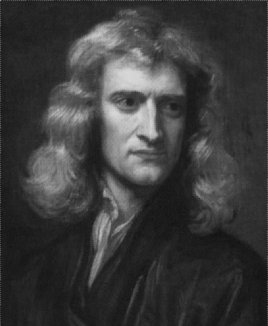
\includegraphics[width=0.25\textwidth]{figures/Newton}
  \end{flushright}
  \vspace*{-4cm}
  \begin{block}{Standard form of a nonlinear system}
    \[ F(u) = 0 \]
  \end{block}
  
  \begin{block}{Iteration}
    \begin{align*}
      \text{Solve:} & \qquad J(u) w = -F(u) \\
      \text{Update:} & \qquad u^+ \gets u + w
    \end{align*}
    \begin{itemize}
    \item Quadratically convergent near a root: $|u^{n+1}-u^*| \in \mathcal{O} \Big(|u^n-u^*|^2\Big)$
    \item Picard is the same operation with a different $J(u)$
    \end{itemize}
  \end{block}
  
%\begin{block}{Nonlinear Poisson}
%    \begin{align*}
%      F(u)=0 \quad &\sim\quad -\div\big[ (1+u^2) \grad u \big] - f = 0 \\
%      J(u)w \quad &\sim\quad  -\div\big[(1+u^2)\grad w + 2uw\grad u \Big]
%    \end{align*}
%\end{block}
\end{frame}



\begin{frame}[fragile]{PETSc Solvers}

\begin{block}{Nonlinear Solvers - Newton and Picard Methods}
\begin{itemize}
  \item Using PETSc linear algebra, just add:
  \begin{lstlisting}[basicstyle=\footnotesize\ttfamily]
SNESSetFunction(SNES snes, Vec r, residualFunc, void *ctx)
SNESSetJacobian(SNES snes, Mat A, Mat M, jacFunc, void *ctx)
SNESSolve(SNES snes, Vec b, Vec x)
  \end{lstlisting}

  \item Can access subobjects
  \begin{lstlisting}[basicstyle=\footnotesize\ttfamily]
SNESGetKSP(SNES snes, KSP *ksp)
  \end{lstlisting}

  \item Can customize subobjects from the cmd line
  \begin{itemize}
    \item Set the subdomain preconditioner to ILU with \lstinline|-sub_pc_type ilu|
  \end{itemize}
\end{itemize}
\end{block}

\end{frame}
